\chapter{Compilation}

\section{Dynamic Memory Management}
Native support of complex data structures is not a trivial matter to implement in a reversible computing environment. Variable-sized records and frames needs to be stored efficiently in a structured heap, while avoiding garbage build-up to maintain reversibility. A reversible heap manager layout has been proposed for a simplified version of the reversible functional language \textsc{RFun} and later expanded to allow references to avoid deep copying values~\cite{ha:heap, ty:rfun, tm:refcounting}.

The following section presents a discussion of various heap manager layouts along with their advantages and disadvantages in terms of implementation difficulty, garbage build-up and the OOP domain. 

\subsection{Heap manager layout}
Heap managers can be implemented in numerous ways. Different layouts yield advantages when allocating memory, finding a free block or when collecting garbage. As our goal is to construct a garbage-free heap manager, our finalized design should emphasize and reflect this objective in particular. Furthermore, we should attempt to allocate and deallocate memory as efficiently as possible, as merging blocks would be a non-reversible action.

\subsubsection{Memory Pools}
A simple layout for a heap manager would allocate memory using fixed-size blocks regardless of the actual size of the record~\cite{bk:memorypool}. This would simplify the implementation greatly as the free list simply is a linked list of free cells of identical size. However, a huge disadvantage to this approach is large amounts of garbage is generated due to fragmentation.

\subsubsection{Buddy Memory}
In this approach we have all blocks be variable-size of the power-of-two. Having different block sizes and methods for splitting a larger block into smaller ones reduces fragmentation. In terms of implementation, reversible splitting and merging might be possible as we're always doubling the size when merging and halving when splitting, thus making the operations logically inverse of each other~\cite{dk:buddyalloc}.

\subsubsection{One heap per record}
Another layout approach would be maintaining one heap per record in the program. During compilation classes would be analysed and a heap for each class would be created. The advantage of this approach would be less garbage generation as each allocation is tailored as closely as possible to the size of the record obtained from a static analysis during compilation. The obvious disadvantage is the amount of book-keeping and workload associated with growing and shrinking a heap and its neighbours.

\subsubsection{Shared heap, record-specific free lists}
A combination of the previous layouts would consist of a single heap, but record-specific free lists. This way, we ensure minimal fragmentation when allocating and freeing as the different free lists ensures that allocation of an object wastes as little memory as possible. By only keeping one heap, we eliminate the growth/shrinking issues of the multiple heap layout. There is however still a considerable amount of book-keeping involved in maintaining multiple free-lists. The bigger the number of unique classes defined in a program, the more free-lists we need to maintain during execution. If the free-lists are not allowed to point at the same free block (which they intuitively shouldn't in order to ensure reversibility), programs with many classes, say one hundred, could potentially fill up the heap with one hundred free lists, but only ever allocate objects for one of the classes, thus wasting a lot of memory on unused free lists. This scenario could potentially be avoided with compiler optimizations.\\

\subsubsection{Other layouts to consider (?)}
\texttt{Idea: Slab-like allocation}

\begin{figure}
  \centering
  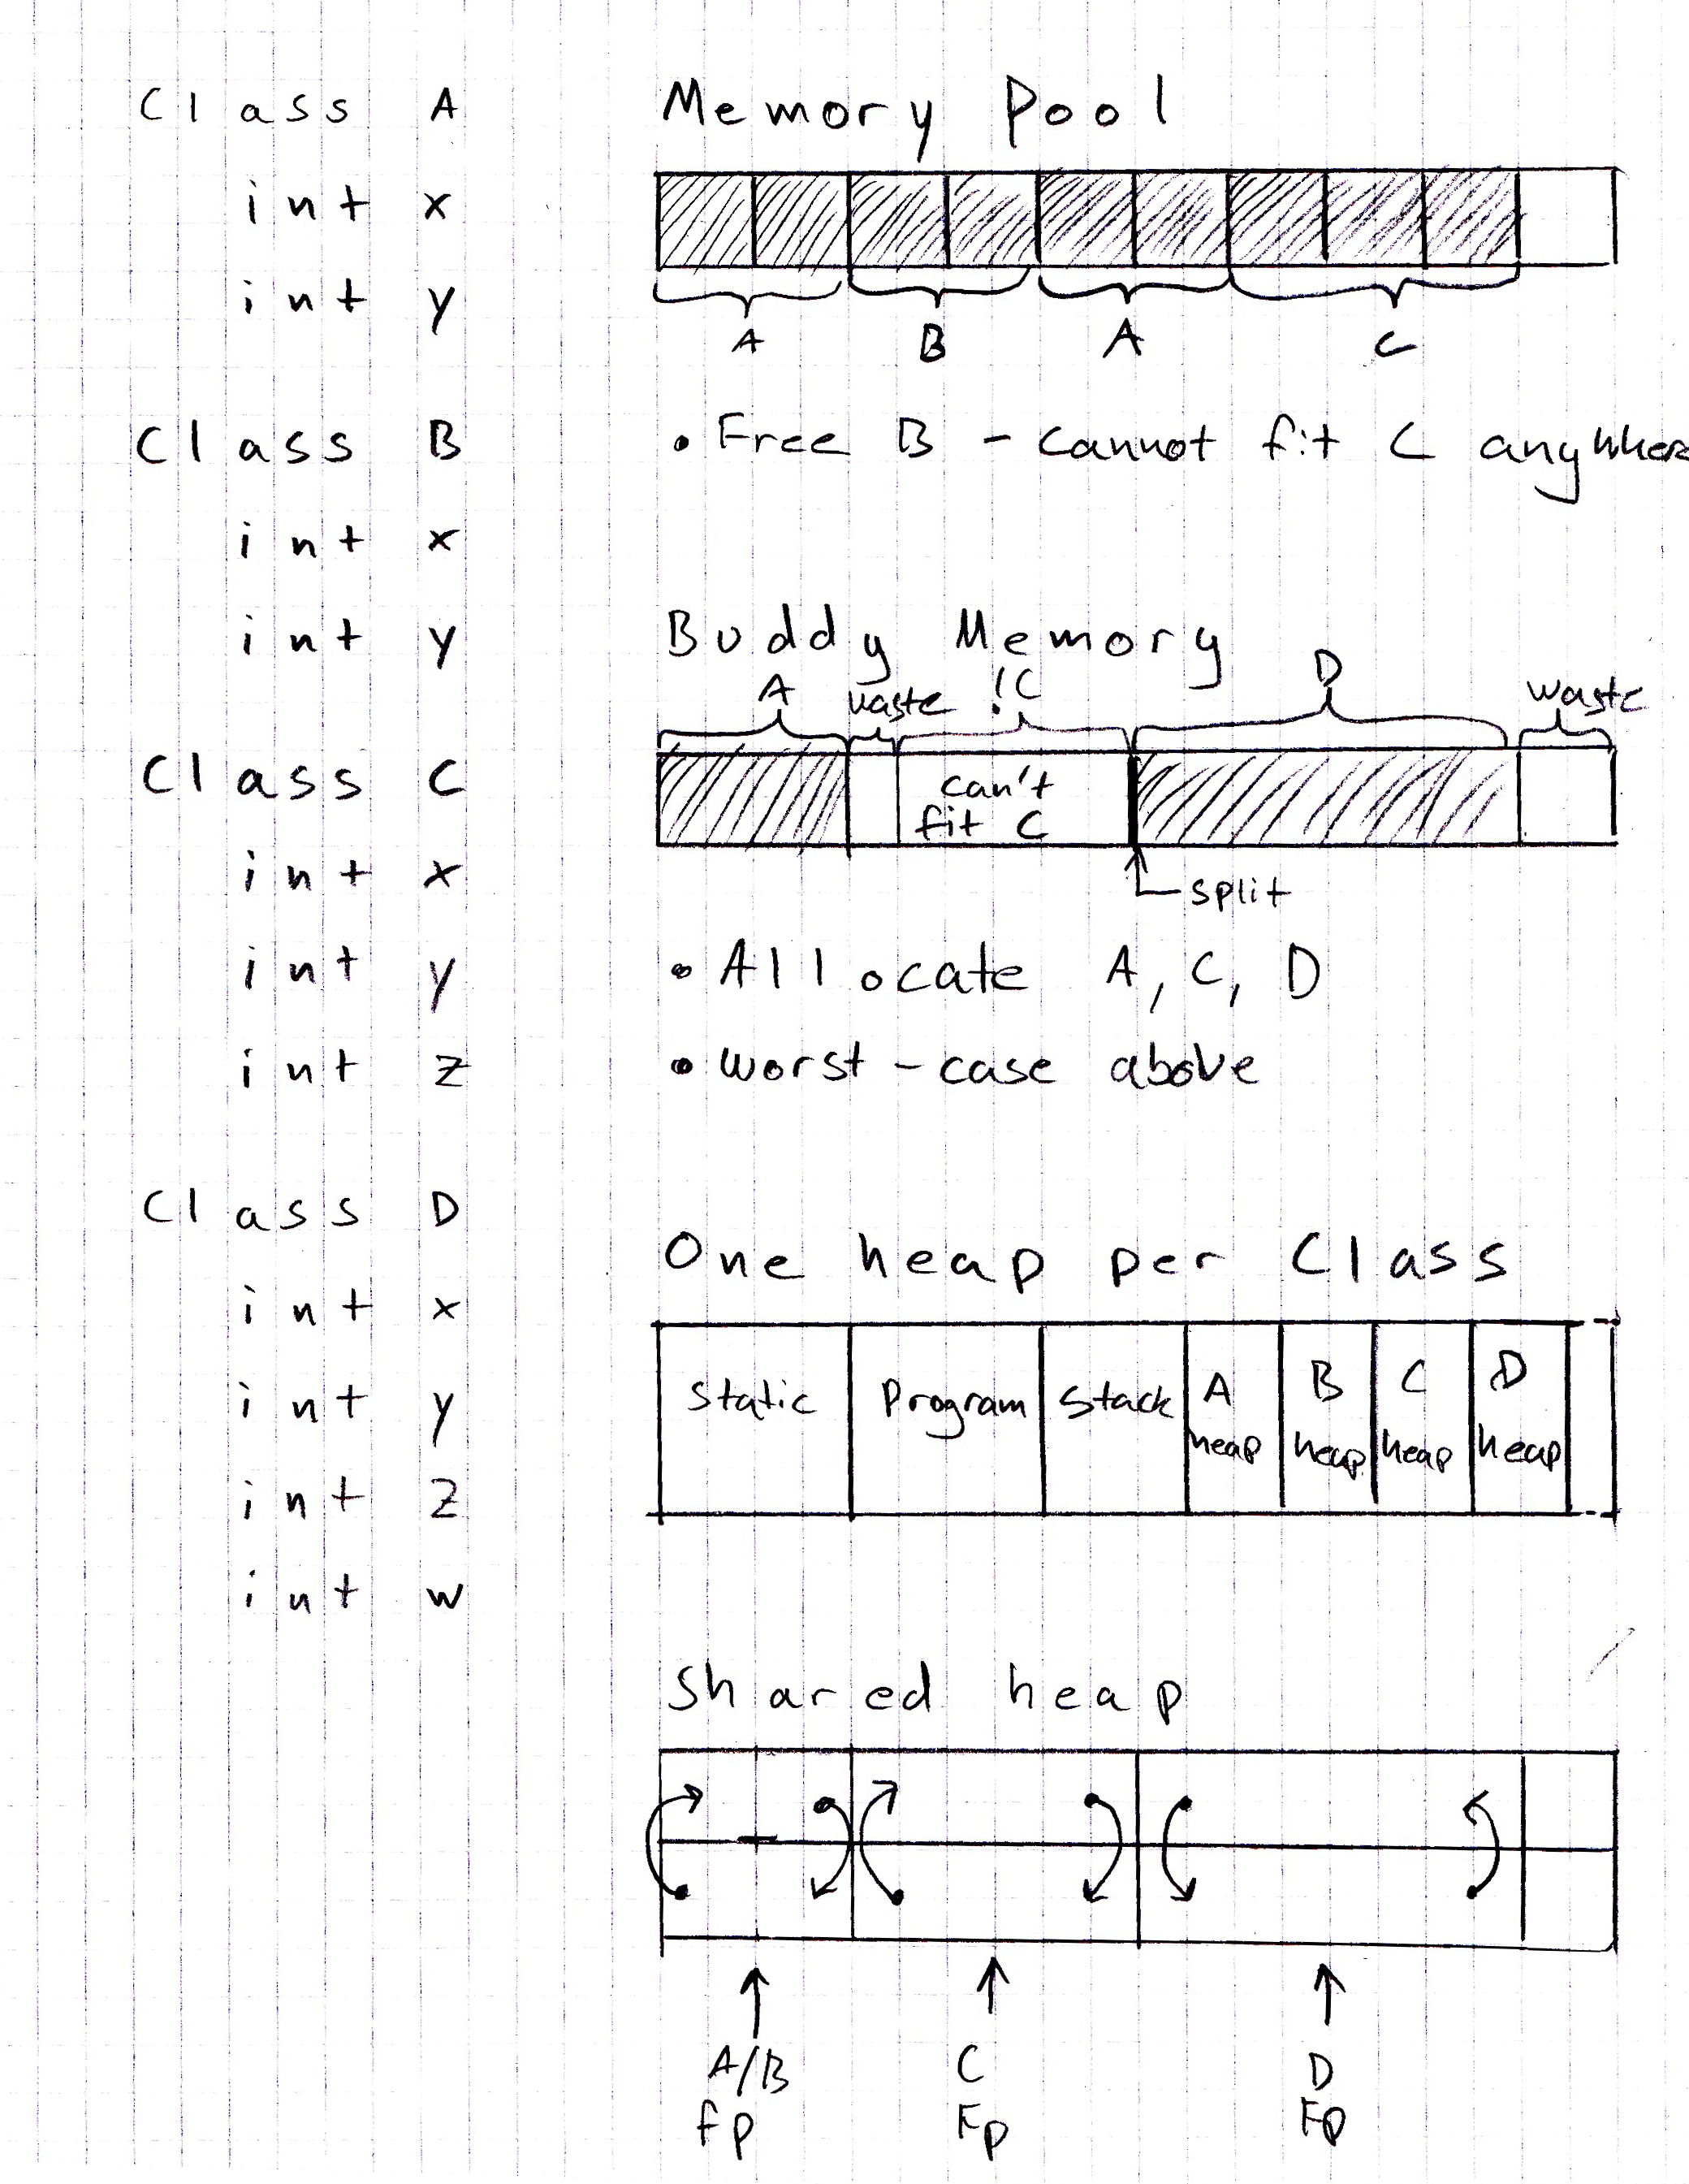
\includegraphics[width=0.7\textwidth]{heap-designs}
  \caption{Heap memory layouts (Draft)}
\end{figure}
